%% LyX 2.0.6 created this file.  For more info, see http://www.lyx.org/.
%% Do not edit unless you really know what you are doing.
\documentclass[english]{beamer}
\usepackage{mathptmx}
\usepackage[T1]{fontenc}
\usepackage[latin9]{inputenc}
\usepackage{amsmath}
\usepackage{amssymb}
\usepackage{minted}
\usepackage[cmtip,all]{xy}
\newcommand{\longsquiggly}{\xymatrix{{}\ar@{~>}[r]&{}}}


\makeatletter
%%%%%%%%%%%%%%%%%%%%%%%%%%%%%% Textclass specific LaTeX commands.
 % this default might be overridden by plain title style
 \newcommand\makebeamertitle{\frame{\maketitle}}%
 \AtBeginDocument{
   \let\origtableofcontents=\tableofcontents
   \def\tableofcontents{\@ifnextchar[{\origtableofcontents}{\gobbletableofcontents}}
   \def\gobbletableofcontents#1{\origtableofcontents}
 }
 % plain title style, override default
 \renewcommand\makebeamertitle{\frame[plain]{\maketitle}}%
 \long\def\lyxframe#1{\@lyxframe#1\@lyxframestop}%
 \def\@lyxframe{\@ifnextchar<{\@@lyxframe}{\@@lyxframe<*>}}%
 \def\@@lyxframe<#1>{\@ifnextchar[{\@@@lyxframe<#1>}{\@@@lyxframe<#1>[]}}
 \def\@@@lyxframe<#1>[{\@ifnextchar<{\@@@@@lyxframe<#1>[}{\@@@@lyxframe<#1>[<*>][}}
 \def\@@@@@lyxframe<#1>[#2]{\@ifnextchar[{\@@@@lyxframe<#1>[#2]}{\@@@@lyxframe<#1>[#2][]}}
 \long\def\@@@@lyxframe<#1>[#2][#3]#4\@lyxframestop#5\lyxframeend{%
   \frame<#1>[#2][#3]{\frametitle{#4}#5}}
 \newenvironment{topcolumns}{\begin{columns}[t]}{\end{columns}}
 \def\lyxframeend{} % In case there is a superfluous frame end

%%%%%%%%%%%%%%%%%%%%%%%%%%%%%% User specified LaTeX commands.
\usetheme{Kitware}

\makeatother

\usepackage{babel}
\begin{document}





\title[CastXML]{Wrapping C and C++ Libraries with CastXML}


%\subtitle{Include Only If Paper Has a Subtitle}


\author[King, Brad]{Brad~King\inst{1}, Bill Hoffman\inst{1}, Matt
McCormick\inst{1}, and Michka Popoff}


\institute[Kitware, Inc]{\inst{1}Kitware, Inc.}


\date[2015-07-10]{SciPy, 2015}

\makebeamertitle


\AtBeginSubsection[]{

  \frame<beamer>{

    \frametitle{Outline}

    \tableofcontents[currentsection,currentsubsection]

  }

}




%\beamerdefaultoverlayspecification{<+->}


\lyxframeend{}\lyxframe{Outline}

\tableofcontents{}




\lyxframeend{}\section{Motivation and History}



\lyxframeend{}\subsection[Wrapping ITK]{Wrapping the Insight Toolkit (ITK)}

\lyxframeend{}\lyxframe{The Insight Toolkit (ITK)}

\begin{itemize}

  \item In 1999, the US National Institute of Health's (NIH) National Library
    of Medicine (NLM) started a project to support the Visible Human Project.

\end{itemize}

\begin{columns}
  \column{0.5\textwidth}
  
\includegraphics[width=4cm]{images/VisibleHuman}
  \column{0.5\textwidth}
  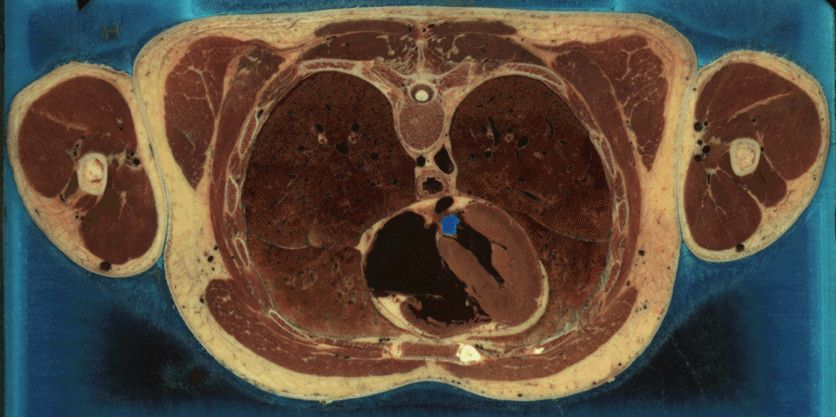
\includegraphics[width=4.7cm]{images/VisibleSlice}
\end{columns}


\lyxframeend{}\lyxframe{Image Segmentation}

\begin{columns}
  \column{0.5\textwidth}
  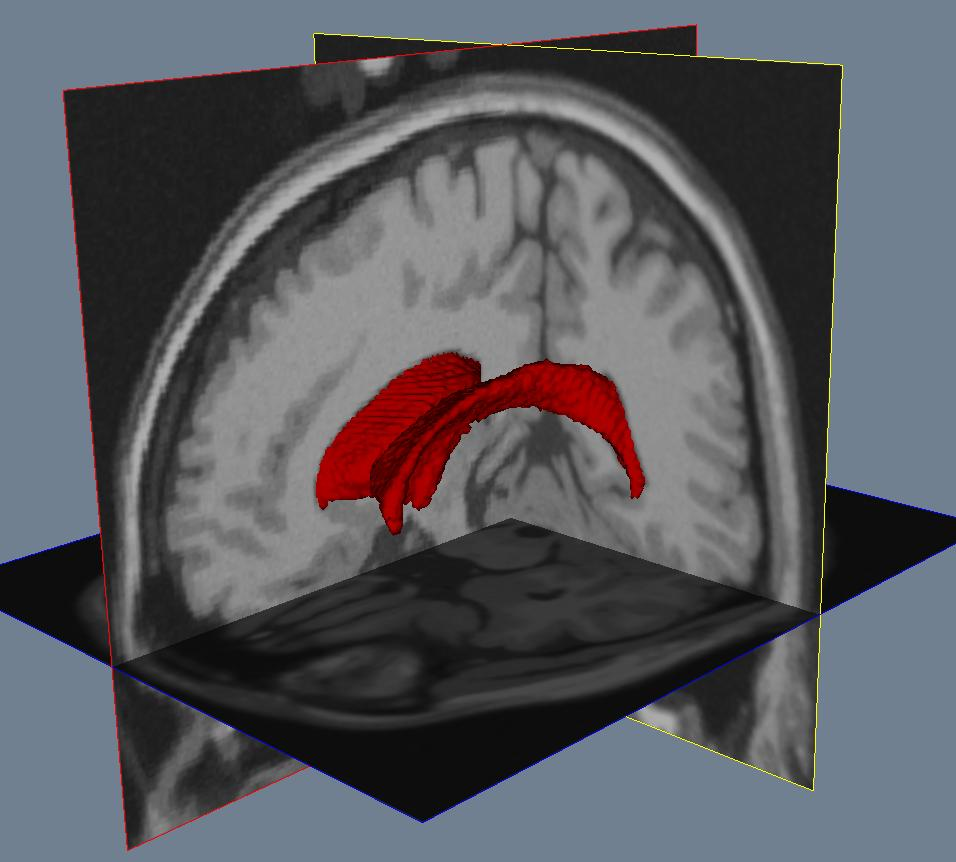
\includegraphics[width=5cm,height=4cm]{images/VentricleSegmentation}
  \column{0.5\textwidth}
  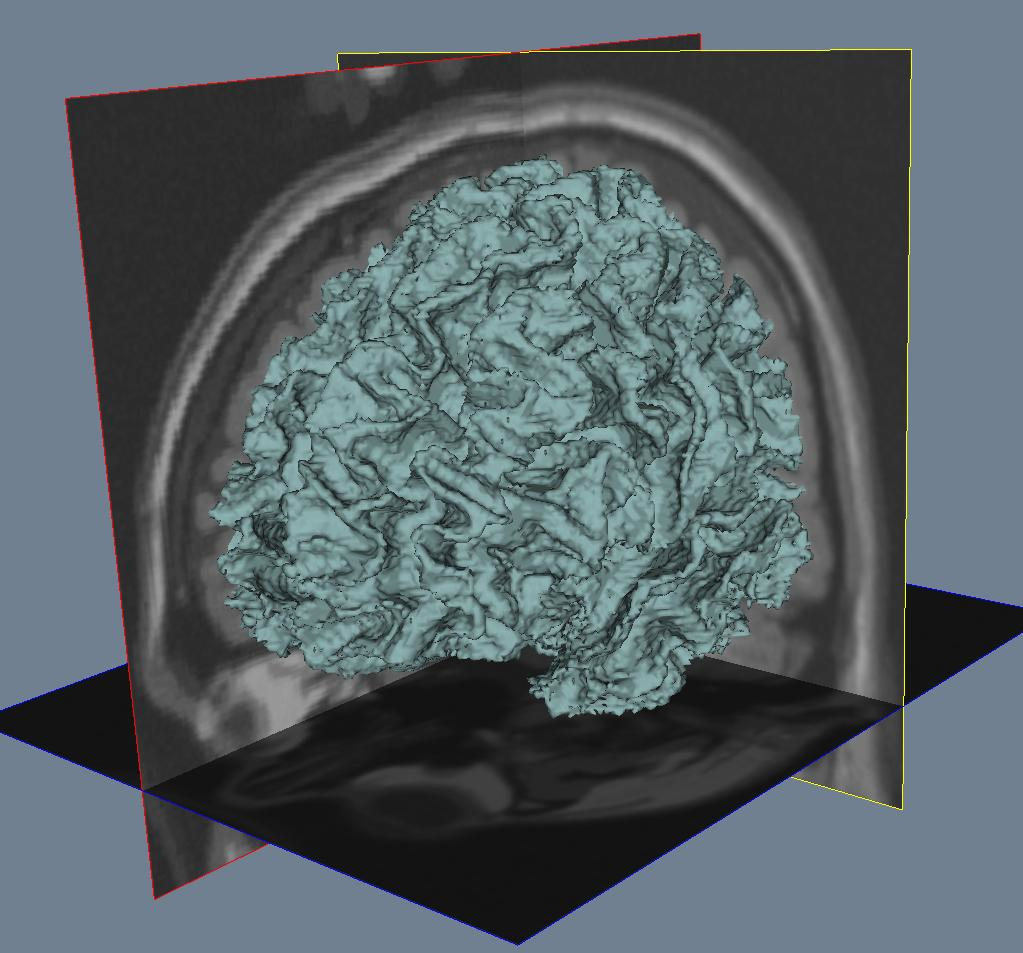
\includegraphics[width=5cm,height=4cm]{images/WhiteMatterSegmentation}
\end{columns}


\lyxframeend{}\lyxframe{Image Registration}

\begin{columns}
  \column{0.5\textwidth}
  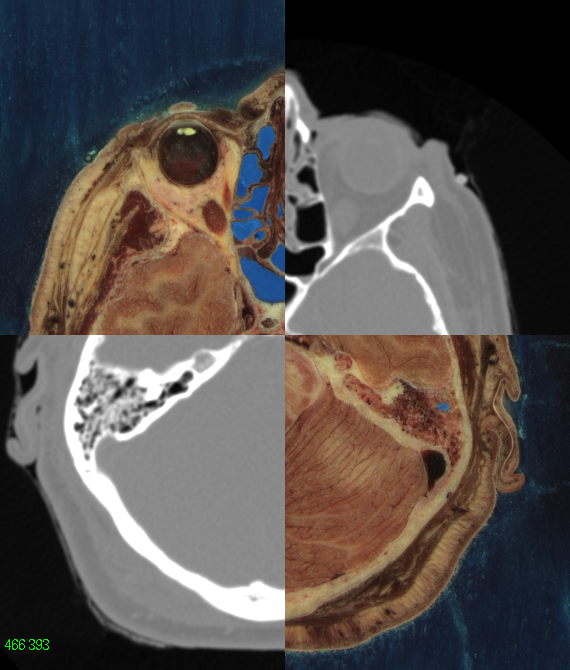
\includegraphics[width=5cm]{images/Registration1}
  \column{0.5\textwidth}
  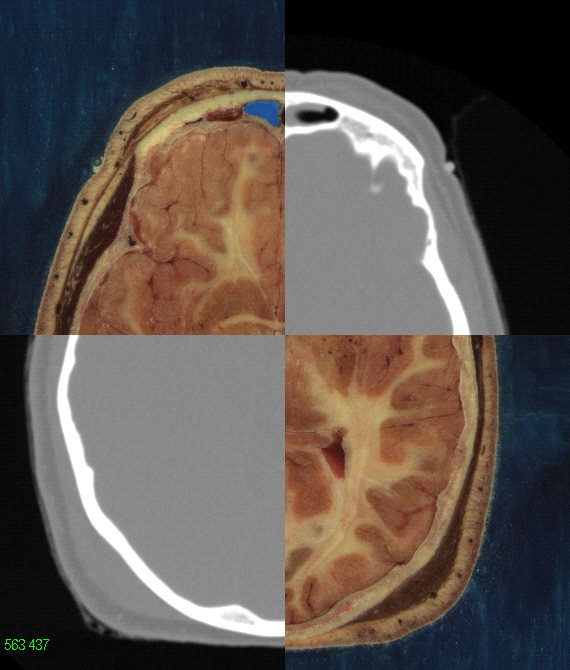
\includegraphics[width=5cm]{images/Registration2}
\end{columns}


\lyxframeend{}\lyxframe{Large C++ Codebase}

\begin{itemize}
  \item<1-> Development has progressed since 1999
  \item<2-> Over \alert{1.6 million} lines of code
  \item<3-> Highly templated C++
\end{itemize}

\begin{figure}
  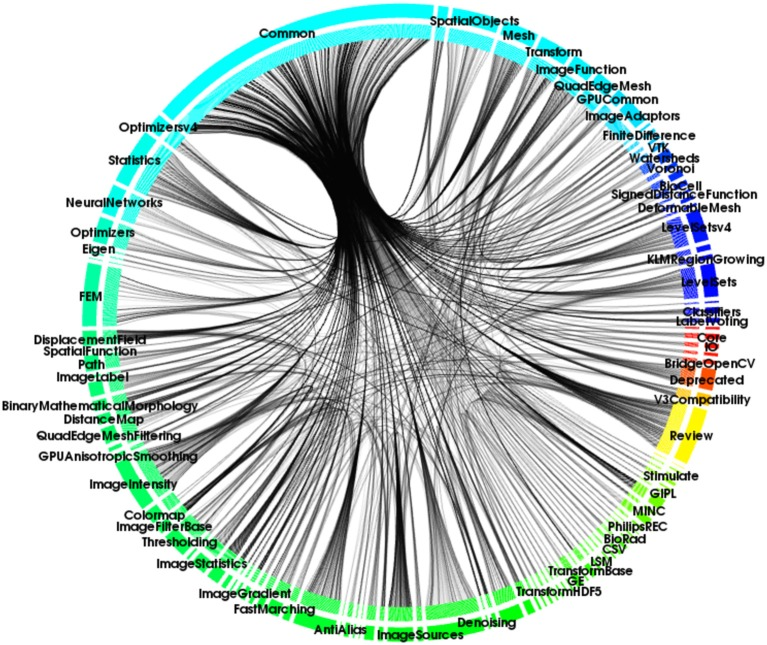
\includegraphics[width=4cm]{images/Modules}
  \caption{Visualization of the toolkit modules.}
\end{figure}


\lyxframeend{}\lyxframe{We Want to Use Python!}

\centerline{
\includegraphics[height=7cm]{images/WrapITK}}


\lyxframeend{}\lyxframe{ITK's Wrapping Process}

\begin{enumerate}
  \item<1-> \alert<5->{Determine an Abstract Syntax Tree (AST)} from C++ sources
  \item<2-> Create Swig \texttt{.i} from the AST and desired template
    parameters
  \item<3-> Generate CPython extension modules code with Swig
  \item<4-> Build the extension modules
\end{enumerate}



\lyxframeend{}\subsection[C++ AST]{Generating an Abstract Syntax Tree (AST)}


\lyxframeend{}\begin{frame}[fragile]{C++ Source Code to Abstract Syntax Tree}

\begin{columns}
  \column{0.3\textwidth}
  \begin{minted}[fontsize=\tiny]{cpp}
  namespace MyCoolProject {
    struct test_results {
      enum status {
        ok,
        fail,
        error
      };
      void update(
        const char * test_name,
        status result );
    };
  }
  \end{minted}
  \column{0.2\textwidth}
\only<2>{
  \Huge
  $\mathbf{\longrightarrow}$
  \normalsize
}
\only<3->{
  \Huge
  $\mathbf{\longsquiggly}$
  \normalsize
}
  \normalsize
\only<2->{
Process and parse
}
  \column{0.3\textwidth}
  \begin{minted}[fontsize=\tiny]{cpp}
<?xml version="1.0"?>
<GCC_XML version="0.9.0" cvs_revision="1.136">
  <Namespace id="_5" name="MyCoolProject" context="_1" members="_9"/>
  <ArrayType id="_8" min="0" max="0" type="_10"/>
  <Struct id="_9" name="test_results" context="_5" location="f1:2" file="f1" line="2" members="_11 _12 _13 _14 _15 _16" size="8" align="8"/>
  <Typedef id="_10" name="__va_list_tag" type="_17" context="_1" location="f0:0" file="f0" line="0"/>
  <Enumeration id="_11" name="status" context="_9" access="public" location="f1:3" file="f1" line="3">
    <EnumValue name="ok" init="0"/>
    <EnumValue name="fail" init="1"/>
    <EnumValue name="error" init="2"/>
  </Enumeration>
  <Method id="_12" name="update" returns="_18" context="_9" access="public" location="f1:8" file="f1" line="8" mangled="_ZN13MyCoolProject12test_results6updateEPKcNS0_6statusE">
    <Argument name="test_name" type="_19" location="f1:9" file="f1" line="9"/>
    <Argument name="result" type="_11" location="f1:10" file="f1" line="10"/>
  </Method>
  ...
</GCC_XML>
  \end{minted}
\end{columns}

\only<4->{
  \centerline{
\includegraphics[height=4cm]{images/LabyrinthCropped}}

  \tiny
  Image source:
  https://en.wikipedia.org/wiki/Labyrinth\_%28film%29#/media/File:Labyrinth\_ver2.jpg
  \normalsize
}
\end{frame}


\lyxframeend{}\lyxframe{The C++kie Model}

\begin{columns}
  \column{0.25\textwidth}
\only<1->{
  C++ Source Code
  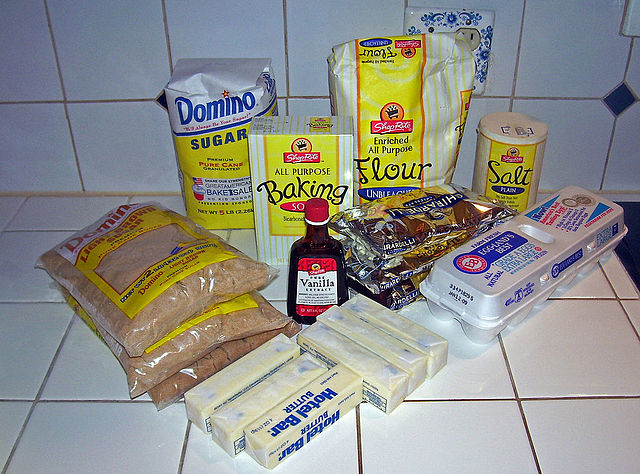
\includegraphics[width=2cm]{images/Ingredients}
}
  \column{0.1\textwidth}
\only<2->{
  $\mathbf{\longsquiggly}$
}
  \column{0.25\textwidth}
\only<2->{
  Abstract Syntax Tree
  
\includegraphics[width=2cm]{images/Gingerbread}
}
  \column{0.1\textwidth}
\uncover<3->{
  $\mathbf{\longrightarrow}$
}
  \column{0.25\textwidth}
\only<3->{
  Python Wrappers
  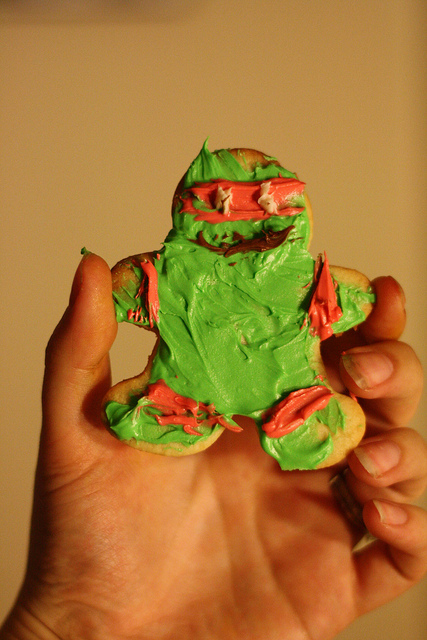
\includegraphics[width=2cm]{images/NinjaGingerbread}
}
\end{columns}

%\tiny
%Image sources:

%https://www.flickr.com/photos/ginnerobot/4516934176

%http://yuzumilk.exblog.jp/17080398

%https://en.wikipedia.org/wiki/Chocolate\_chip\_cookie\#/media/File:Chocolate\_chip\_cookie\_ingredients.jpg

%\normalsize


\lyxframeend{}\lyxframe{AST Generation Complexity}

\begin{columns}
  \column{0.25\textwidth}
\only<1->{
  C++ Source Code
  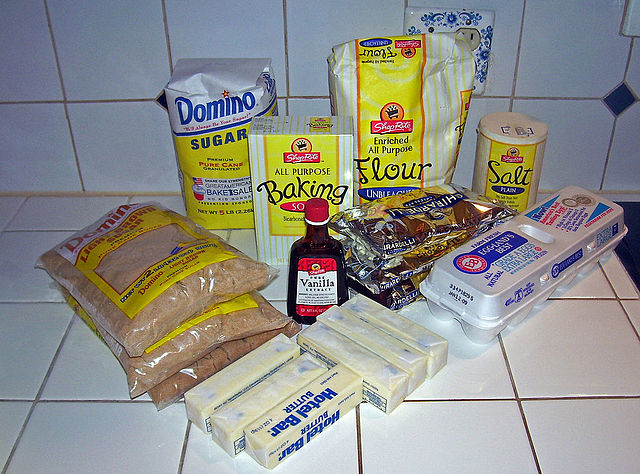
\includegraphics[width=2cm]{images/Ingredients}
}
  \column{0.05\textwidth}
\only<2->{
  $\mathbf{\longrightarrow}$
}
  \column{0.35\textwidth}
\only<2->{
  Processing
}
  \begin{itemize}
    \item<3-> C preprocessor
    \item<4-> Standard library headers (compiler specific)
    \item<5-> Compiler flags
  \end{itemize}

\only<2->{
  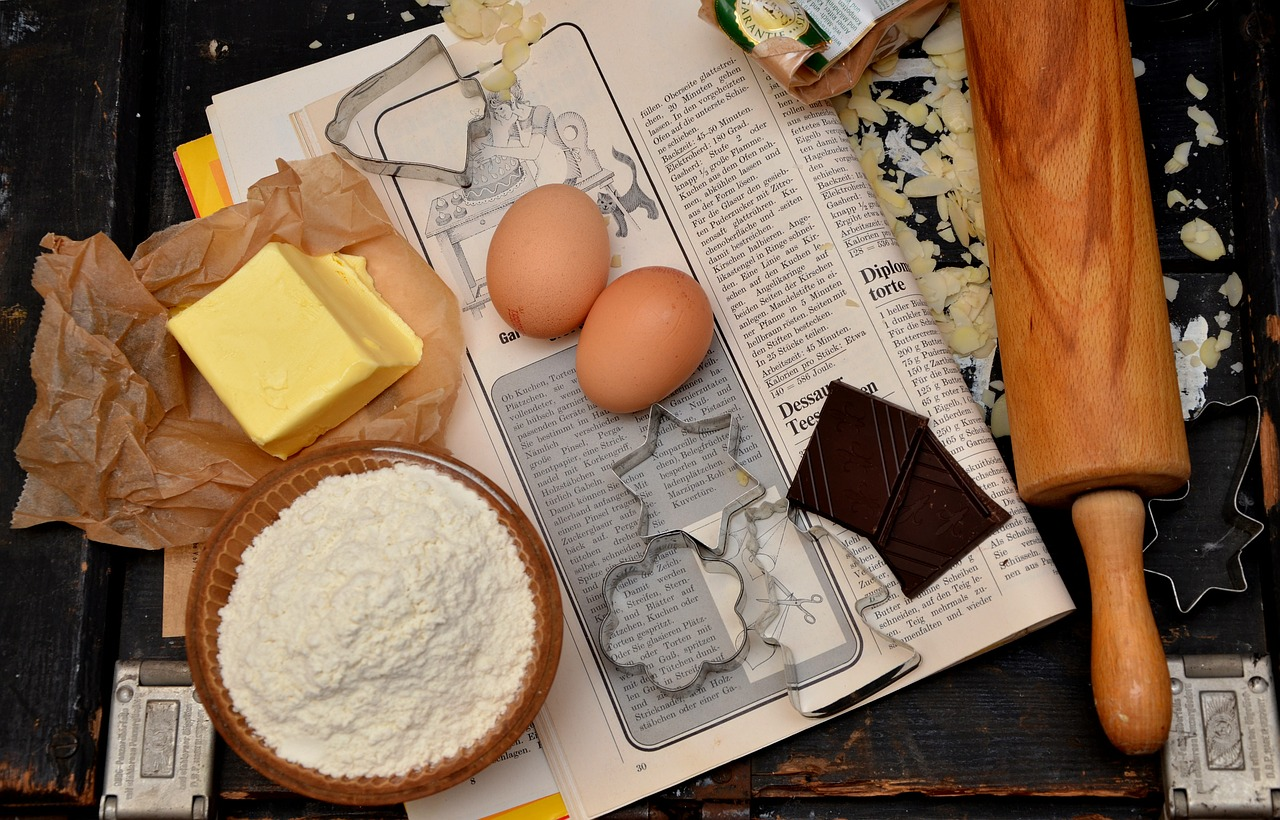
\includegraphics[width=3cm]{images/Bake}
  % image source:https://pixabay.com/p-525226/?no_redirect
}

  \column{0.05\textwidth}
\uncover<3->{
  $\mathbf{\longrightarrow}$
}
  \column{0.25\textwidth}
\only<6->{
  Abstract Syntax Tree
  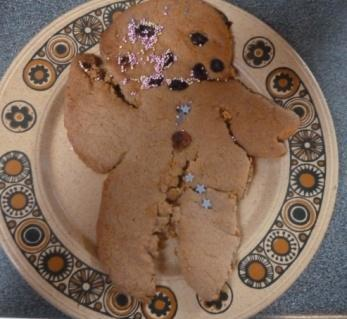
\includegraphics[width=3cm]{images/DavidsGingerbread}
  % Image source:
  % http://i431.photobucket.com/albums/qq32/ali991/Gingerbread_zps82331c17.jpg
}
\end{columns}

\only<6->{
  \centerline{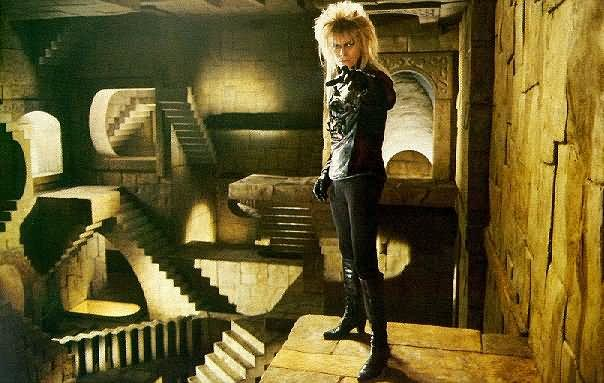
\includegraphics[width=5cm]{images/Bowie}}
  %image source:
%http://s3.amazonaws.com/quietus_production/images/articles/1850/bowie_labyrinth_1245071926.jpg
}




\lyxframeend{}\subsection[GCC-XML]{GCC-XML}


\lyxframe{GCC-XML}

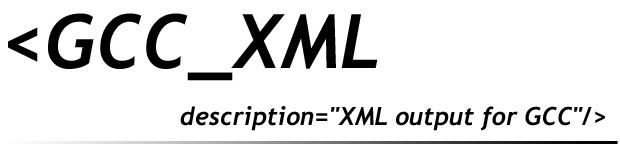
\includegraphics[height=1.8cm]{images/GccXml.png}

\begin{itemize}
  \item<2->Does C preprocessing
  \item<3->Uses standard library headers of the simulated compiler
  \item<4->Uses compiler flags for simulated compiler
  \item<5->Uses GCC's C++ parsing capabilities
  \item<6->Generates XML AST representation
\end{itemize}


\lyxframeend{}\lyxframe{General Projects That Also Used GCC-XML}


\begin{columns}

  \column{0.5\textwidth}
  \begin{itemize}
   \item<1->Pyste (Boost.Python)
   \item<2->Py++ (Boost.Python)
   \item<3->Python ctypeslib
   \item<4->xdress
   \item<5->Others...
  \end{itemize}

  \column{0.5\textwidth}

  \begin{center}
  \only<1->{

\includegraphics[width=4cm]{images/Boost.png}
}
  \only<4->{
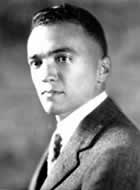
\includegraphics[width=2cm]{images/Hoover.png}
}
\end{center}
\end{columns}


\lyxframeend{}\lyxframe{GCC-XML's Weakness}

\begin{center}
\Huge
\only<2->{Maintainability.}
\normalsize
\end{center}


\lyxframeend{}\section{CastXML Description}

\lyxframeend{}\lyxframe{CastXML}

CastXML is a GCC-XML replacement that uses LLVM/Clang.

\begin{block}{CastXML}
A \textbf{C}-family \textbf{a}bstract \textbf{s}yntax
\textbf{t}ree \textbf{XML} output tool.
\end{block}


\lyxframeend{}\subsection{Building}

\lyxframeend{}\lyxframe{CastXML}

Building requires

\begin{itemize}
  \item<1-> A C++ compiler with C++11 support
  \item<2-> CMake
  \item<3-> LLVM/Clang 3.6.0 or later. Currently must be
    \begin{itemize}
      \item Built from source
      \item Installed into an install prefix
    \end{itemize}
\end{itemize}

\begin{columns}

  \column{0.5\textwidth}

  \begin{center}
  \only<2->{

\includegraphics[width=4cm]{images/CMake.png}
}
\end{center}
  \column{0.5\textwidth}

  \begin{center}
  \only<3->{

\includegraphics[width=4cm]{images/Clang.png}
}
\end{center}
\end{columns}





\lyxframeend{}\lyxframe{Invocation}

\lyxframeend{}\subsection{Invocation}

\begin{block}{Invocation}
  \begin{verbatim}
castxml \
  --castxml-gccxml \
  --castxml-cc-msvc cl \
  -o ouput.xml
  input.cxx
  \end{verbatim}
\end{block}

\lyxframeend{}\section{SciPy Ecosystem Integration}


\lyxframeend{}\subsection{pygccxml}

\lyxframeend{}\lyxframe{pygccxml}

\begin{block}{pygccxml}
A specialized XML reader that reads the output from CastXML and GCC-XML. It
provides a simple framework to navigate C++ declarations using Python classes.
\end{block}

Repository: \url{https://github.com/gccxml/pygccxml}


\lyxframeend{}\lyxframe{pygccxml History}

\begin{itemize}
  \item<1-> The original author is Roman Yakovenko (2004-2011).
  \item<2-> Forked multiple times by different authors to add Python 3
    support.
  \item<3-> In May 2014, Michka Popoff and the Insight Software Consortium
    revived pygccxml.
\end{itemize}


\lyxframeend{}\lyxframe{New since 2014}

\begin{itemize}
  \item Mercurial to Git
  \item Travis-ci.org hook for Python 2.6, 2.7, 3.2, 3.3, 3.4
    support.
  \item coverall.io hook for code coverage
  \item Docs on readthedocs.org
  \item quantifiedcode.com hook for code structure
  \item PEP8 compatible
\end{itemize}


\lyxframeend{}\section*{Summary}


\lyxframeend{}\lyxframe{Summary}

\begin{itemize}
  \item Generating an \alert{Abstract Syntax Tree} is an important part of the wrapping
  process.
  \item The Abstract Syntax Tree is \alert{compiler-dependent} because of the C
    preprocessor, standard library headers, and 
lines.
\item \alert{CastXML} captures the compiler-dependence and does complex parsing of C++.
\item \alert{pygccxml} is a Python interface to CastXML output
\end{itemize}


\lyxframeend{}

\lyxframeend{}\section*{Appendix}


\lyxframeend{}\subsection*{Resources}


\lyxframeend{}\lyxframe{[allowframebreaks]Resources}

\begin{center}
\small
\begin{description}
  \item[Mailing list] \hfill \\ \url{http://public.kitware.com/mailman/listinfo/castxml}
  \item[Repository] \hfill \\ \url{https://github.com/CastXML/CastXML}
\end{description}
\normalsize
\end{center}

\beamertemplatebookbibitems

\lyxframeend{}
\end{document}
